\chapter{Analyse des besoins et conception}
\begin{spacing}{1.2}
\minitoc
\thispagestyle{MyStyle}
\end{spacing}
\clearpage

\section{Introduction}

Après le cadre général du projet et les concepts fondamentaux, ce chapitre formalise les
besoins de la plateforme et pose les bases de sa conception. Nous identifions les acteurs
puis les exigences fonctionnelles et non fonctionnelles, avant de proposer une
modélisation UML (vues fonctionnelle, structurelle et dynamique) complétée par une
architecture globale. Nous décrivons enfin les capacités d'intelligence artificielle qui
distinguent la plateforme et les choix de modèles de ses agents spécialisés.

\section{Analyse des besoins}

\subsection{Identification des acteurs}

La plateforme s'adresse à deux acteurs principaux~: l'\textbf{Ingénieur DevOps} et
l'\textbf{Administrateur}. Ce périmètre reflète l'usage réel observé pendant le
développement~: un outil de travail pour l'ingénieur qui automatise la conception et le
déploiement d'une infrastructure, complété par un rôle de supervision globale.

\subsubsection{Ingénieur DevOps}

L'ingénieur DevOps est l'utilisateur principal~: il initie un projet, fournit le dépôt
applicatif à analyser et interagit avec le système au fil du workflow. Ses interactions
couvrent l'ensemble du cycle~:

\begin{itemize}
    \item fournir les informations du dépôt cible~;
    \item consulter l'analyse du projet réalisée par les agents~;
    \item examiner les stratégies d'architecture proposées et choisir la plus adaptée à
    ses contraintes~;
    \item valider, ou demander la régénération, des artefacts produits (Dockerfile,
    fichiers Terraform, manifestes Kubernetes, pipelines CI/CD)~;
    \item déclencher les opérations de build, de validation et de planification
    Terraform~;
    \item suivre le workflow en temps réel et approuver, en cas d'échec, les corrections
    proposées par le \textit{Corrector Agent}.
\end{itemize}

Il n'a pas besoin de maîtriser la syntaxe de chaque outil~: la plateforme produit les
artefacts, son rôle étant de guider, valider et arbitrer les décisions importantes.

\subsubsection{Administrateur}

L'administrateur dispose d'une vue transverse et veille au bon fonctionnement général du
système, sans porter sur la conception d'une infrastructure en particulier~:

\begin{itemize}
    \item gérer les projets enregistrés (création, consultation, suppression)~;
    \item suivre l'état des workflows en cours ou terminés, tous projets confondus~;
    \item superviser les artefacts générés et l'historique des exécutions~;
    \item accéder à la configuration du système, notamment les fournisseurs LLM utilisés
    et leur disponibilité.
\end{itemize}

Ce profil correspond à un responsable technique ou un \textit{lead} DevOps souhaitant une
visibilité d'ensemble sur l'utilisation de la plateforme, sans intervenir sur chaque
projet.

\subsection{Exigences fonctionnelles}

Les exigences fonctionnelles sont regroupées par module, en cohérence avec l'architecture
multi-agents~; chaque module correspond à une étape du pipeline DevOps automatisé par la
plateforme.

\begin{itemize}
    \item \textbf{Gestion des projets~:} créer un projet à partir d'un dépôt GitHub,
    consulter son avancement et accéder à l'historique des workflows associés.

    \item \textbf{Analyse du code~:} identifier le langage, le framework, les dépendances
    et les éléments structurants du projet (Dockerfile, fichier de dépendances, base de
    données, etc.).

    \item \textbf{Génération d'architecture~:} proposer plusieurs stratégies cloud
    (\textit{Low Cost}, \textit{Balanced}, \textit{High Performance}) accompagnées d'une
    estimation de coût, et permettre d'en sélectionner une.

    \item \textbf{Génération Docker~:} générer un Dockerfile adapté au projet, en tenant
    compte du langage, du gestionnaire de dépendances et des bonnes pratiques
    d'optimisation d'image.

    \item \textbf{Génération Terraform~:} générer les fichiers Terraform de l'architecture
    sélectionnée, en respectant les conventions HCL et la cohérence entre ressources.

    \item \textbf{Validation Terraform~:} exécuter \texttt{terraform validate} et remonter
    les erreurs éventuelles de syntaxe ou de configuration.

    \item \textbf{Planification Terraform~:} produire un plan (\texttt{terraform plan})
    présentant les ressources créées, modifiées ou supprimées avant tout déploiement réel.

    \item \textbf{Gestion des artefacts~:} conserver les artefacts générés de manière
    persistante, versionnée et associée au projet correspondant.

    \item \textbf{Suivi des workflows~:} suivre en temps réel l'état d'exécution de chaque
    étape (en attente, en cours, terminé, en erreur) et les corrections déclenchées en cas
    d'échec.
\end{itemize}

\subsection{Exigences non fonctionnelles}

Au-delà des fonctionnalités attendues, plusieurs exigences de qualité conditionnent
l'usage réel de la plateforme.

\begin{itemize}
    \item \textbf{Sécurité~:} les artefacts générés respectent les bonnes pratiques de
    sécurité (utilisateurs non-\textit{root} dans les conteneurs, absence de secrets en
    clair, permissions minimales sur les ressources cloud), et les échanges avec les
    fournisseurs LLM n'exposent que les informations strictement nécessaires à la
    génération.

    \item \textbf{Performance~:} les opérations d'analyse et de génération restent dans des
    temps compatibles avec une utilisation interactive, malgré la latence variable des
    appels LLM.

    \item \textbf{Disponibilité~:} un mécanisme de \textit{fallback} entre plusieurs
    fournisseurs LLM limite l'impact des indisponibilités ponctuelles et évite de bloquer
    un workflow en cours.

    \item \textbf{Extensibilité~:} l'architecture multi-agents permet d'ajouter de nouveaux
    agents (nouveau type d'artefact, nouveau fournisseur cloud) sans remettre en cause les
    agents existants.

    \item \textbf{Maintenabilité~:} chaque agent reste responsable d'un périmètre
    clairement délimité, ce qui facilite la correction des anomalies et l'évolution
    indépendante des modules.

    \item \textbf{Traçabilité~:} chaque étape, chaque artefact et chaque correction sont
    enregistrés, afin de reconstituer a posteriori le déroulement d'une exécution.

    \item \textbf{Ergonomie~:} l'interface présente l'avancement du workflow de manière
    claire et progressive, sans exposer l'utilisateur aux détails techniques tant qu'une
    intervention n'est pas nécessaire.
\end{itemize}

\section{Modélisation du système}

Pour passer des exigences à une conception exploitable, nous nous appuyons sur le langage
UML, qui représente le système selon trois vues complémentaires~: la vue fonctionnelle met
en évidence les interactions entre acteurs et système, la vue structurelle décrit
l'organisation des traitements, et la vue dynamique illustre le déroulement temporel des
scénarios représentatifs.

\subsection{Vue fonctionnelle}

\subsubsection{Diagramme global de cas d'utilisation}

\begin{figure}[htbp]
    \centering
    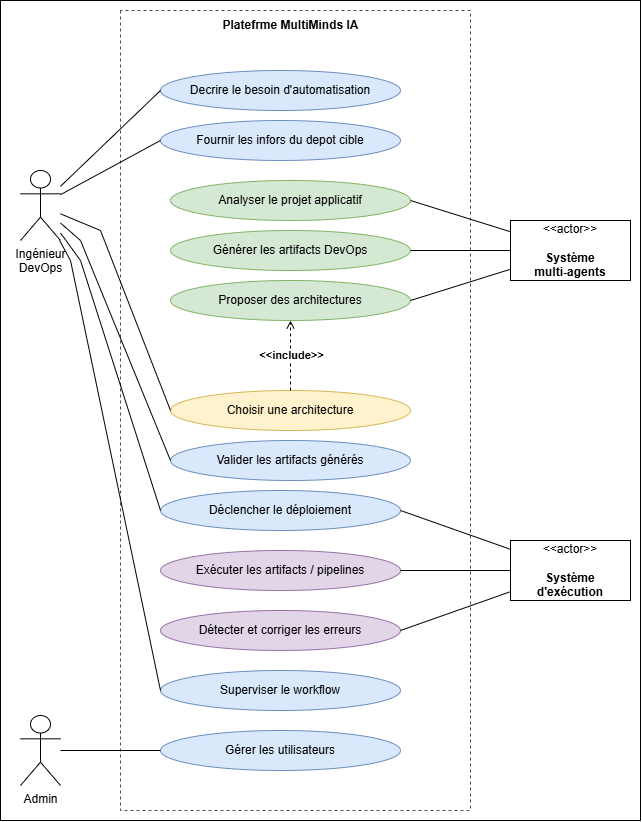
\includegraphics[width=0.85\textwidth]{images/Use_Case_Diagram.png}
    \caption{Diagramme global de cas d'utilisation de la plateforme}
    \label{fig:use-case-global}
\end{figure}

Le diagramme de la figure~\ref{fig:use-case-global} représente les principales
fonctionnalités de la plateforme et les acteurs concernés. L'ingénieur DevOps est l'acteur
déclencheur~: il décrit le besoin d'automatisation et fournit le dépôt cible. Le système
prend ensuite le relais à travers deux sous-systèmes représentés comme acteurs
secondaires~: le \textit{système multi-agents}, responsable de l'analyse du projet, de la
génération des artefacts DevOps et de la proposition d'architectures, et le \textit{système
d'exécution}, responsable de l'exécution des artefacts ainsi que de la détection et de la
correction des erreurs.

Cette représentation matérialise la frontière entre décision humaine et automatisation. Le
cas \textit{Choisir une architecture} est relié par une relation \texttt{<<include>>} au
cas \textit{Proposer des architectures}~: le choix suppose des propositions préalables. De
même, les cas \textit{Valider les artefacts générés} et \textit{Déclencher le déploiement}
placent l'utilisateur en position de contrôle avant toute action irréversible, ce qui
répond au besoin de validation humaine multi-étapes~; enfin, le cas \textit{Détecter et
corriger les erreurs}, porté par le système d'exécution, illustre la boucle de correction
détaillée plus loin.

\subsection{Vue structurelle}

\subsubsection{Diagramme d'activité}

\begin{figure}[htbp]
    \centering
    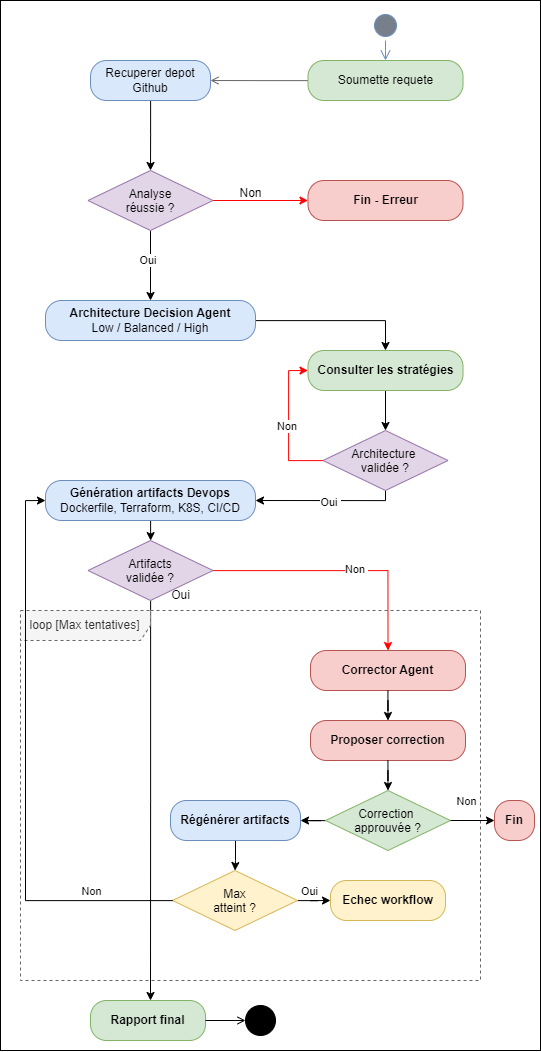
\includegraphics[width=0.62\textwidth]{images/Diag activité.png}
    \caption{Diagramme d'activité~--- déroulement global du workflow}
    \label{fig:activite-workflow}
\end{figure}

La figure~\ref{fig:activite-workflow} décrit l'organisation des traitements, de la
soumission de la requête jusqu'à la production du rapport final. Après récupération du
dépôt GitHub, une première condition vérifie le bon déroulement de l'analyse~; en cas
d'échec, le workflow se termine immédiatement.

Si l'analyse réussit, l'\textit{Architecture Decision Agent} propose plusieurs stratégies
(\textit{Low}, \textit{Balanced}, \textit{High}) que l'utilisateur valide ou non. Tant que
l'architecture n'est pas validée, le workflow revient à l'étape de consultation. Une fois
validée, le système génère les artefacts DevOps (Dockerfile, Terraform, Kubernetes, CI/CD),
à leur tour soumis à validation. En cas d'échec, le \textit{Corrector Agent} propose une
correction~: si elle est approuvée, les artefacts sont régénérés et revalidés, dans la
limite d'un nombre maximal de tentatives~; au-delà, le workflow échoue. Ce diagramme
synthétise ainsi les deux boucles de validation ---~architecture et artefacts~--- qui
structurent le pipeline.

\subsection{Vue dynamique}

\subsubsection{Diagramme de séquence}

\begin{figure}[htbp]
    \centering
    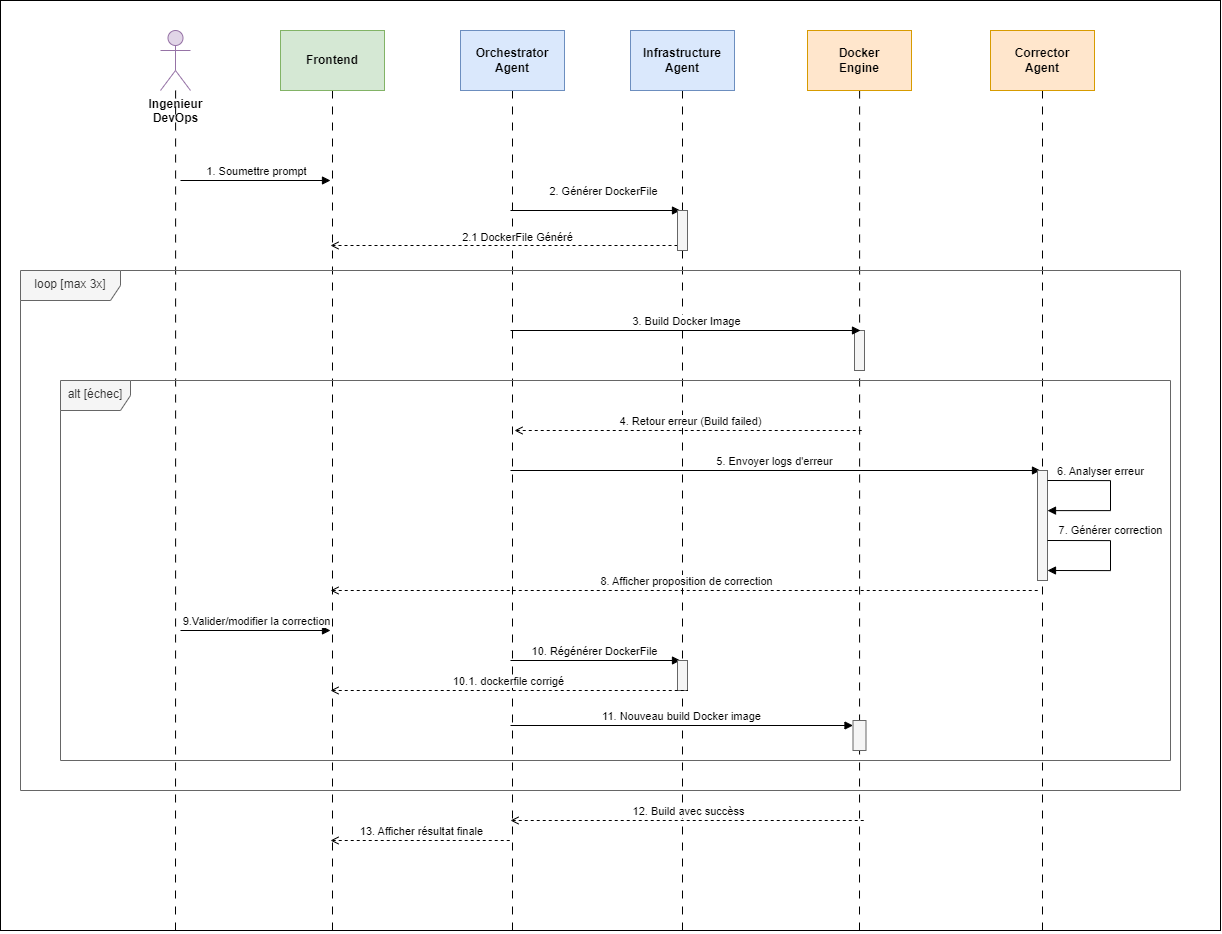
\includegraphics[width=0.90\textwidth]{images/Diag Sequence.png}
    \caption{Diagramme de séquence~--- génération et correction d'un Dockerfile}
    \label{fig:sequence-docker}
\end{figure}

La figure~\ref{fig:sequence-docker} illustre la génération d'un Dockerfile et sa correction
automatique en cas d'échec de build. L'ingénieur DevOps soumet un prompt via le frontend~;
celui-ci est transmis à l'\textit{Orchestrator Agent}, qui sollicite l'\textit{Infrastructure
Agent} pour générer le Dockerfile. Le fichier est ensuite construit par le \textit{Docker
Engine}, à l'intérieur d'une boucle bornée à trois tentatives.

Si le build échoue, l'erreur est remontée à l'orchestrateur, qui transmet les journaux au
\textit{Corrector Agent}. Ce dernier analyse l'erreur et génère une proposition de
correction, que l'ingénieur DevOps valide ou modifie avant régénération et nouveau build.
Lorsque le build aboutit, le résultat remonte à l'utilisateur. Ce scénario met en évidence
un point central de la conception~: la correction n'est jamais totalement automatique, elle
reste soumise à la validation de l'ingénieur, conformément au principe de validation humaine
multi-étapes.

\subsection{Architecture globale de la plateforme}

Les vues précédentes décrivent le système par facettes. La figure~\ref{fig:architecture-globale}
en donne une vision d'ensemble, du frontend jusqu'aux outils DevOps mobilisés le long du
pipeline.

\begin{figure}[htbp]
    \centering
    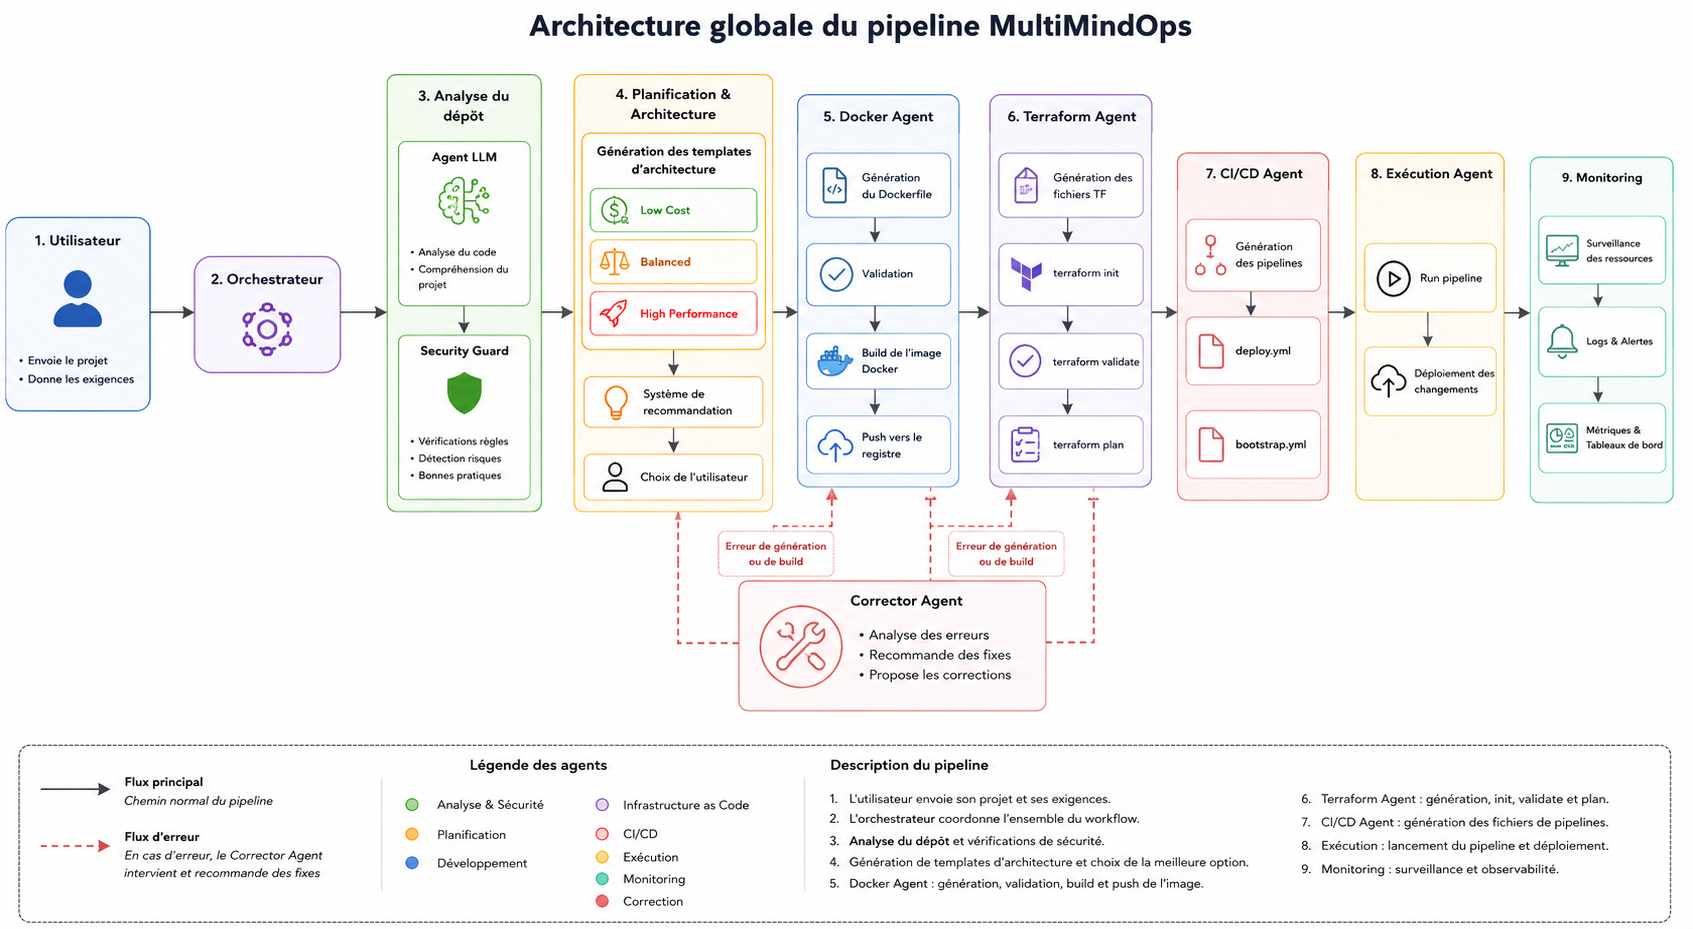
\includegraphics[width=\textwidth]{images/Diag architecture globale.png}
    \caption{Architecture globale de la plateforme MultiMindOps}
    \label{fig:architecture-globale}
\end{figure}

Le frontend communique avec le backend, qui orchestre les agents IA. Ces agents s'appuient
sur une base de connaissances RAG et sur des fournisseurs LLM pour raisonner, puis pilotent
les outils DevOps (Docker, Terraform, CI/CD) afin de produire et d'exécuter les artefacts.
Aux étapes critiques, une validation humaine intervient avant toute action, conformément au
principe \textit{Human-in-the-Loop}.

\section{Aperçu des capacités IA de MultiMindOps}

La valeur de la plateforme repose sur des agents IA spécialisés, chacun dédié à un type
d'artefact DevOps~: la remédiation intelligente des erreurs, la génération d'infrastructure
et la génération de pipelines CI/CD. Ces agents partagent un même socle technique
---~ancrage documentaire par RAG et fournisseur de raisonnement mutualisé~--- que nous
décrivons d'abord, avant de détailler les spécificités métier de chacun.

\subsection{Méthodologie d'évaluation et choix des modèles}

La comparaison qualitative des modèles ne repose pas sur une appréciation subjective, mais
sur la combinaison de plusieurs sources~: les benchmarks publics disponibles dans la
littérature, la documentation officielle des fournisseurs, les expérimentations menées dans
le cadre du projet, et une évaluation automatisée de la qualité des artefacts selon une
approche \textit{LLM-as-a-Judge}~\cite{LLM_AS_JUDGE}, où un modèle de langage note les
sorties d'après une grille prédéfinie. Le score final, exprimé sur~5, correspond à une
moyenne pondérée de plusieurs critères~: qualité des artefacts générés, cohérence
syntaxique, respect des bonnes pratiques, stabilité des réponses, temps de génération et
coût d'utilisation. Les valeurs rapportées dans ce chapitre découlent donc de cette
méthodologie, et non d'une estimation arbitraire.

\subsubsection{Fournisseur de raisonnement mutualisé}

Les trois agents reposent sur une architecture commune, ce qui permet de mutualiser le
choix du fournisseur principal. \textbf{GPT-5-mini} assure la compréhension du contexte, la
génération structurée et le raisonnement. \textbf{Llama~3.3~70B}, hébergé sur Groq,
n'intervient qu'en \textit{fallback} automatique~: il garantit la continuité du service en
cas d'indisponibilité ou de dépassement de quota du fournisseur principal. Ces deux modèles
occupant des rôles distincts~--- principal et secours~--- leur comparaison directe
apporterait peu~; l'analyse comparative est plutôt consacrée à un choix réellement
structurant pour la qualité des réponses~: le modèle d'\textit{embedding} du système RAG.

\subsubsection{Choix du modèle d'embedding pour le RAG}

La pertinence de la récupération documentaire dépend directement du modèle d'\textit{embedding}
retenu. Deux candidats ont été évalués selon la méthodologie précédente~:
\texttt{text-embedding-\allowbreak3-small} (OpenAI) et \texttt{nomic-embed-\allowbreak text-v1.5} (Nomic AI). La
qualité de recherche s'appuie sur les scores publiés du benchmark MTEB~\cite{MTEB}, les
autres critères provenant de la documentation des fournisseurs~\cite{OPENAI_DOCS,NOMIC_EMBED}
et des mesures réalisées dans le projet.

\begin{table}[htbp]
    \centering
    \caption{Comparaison des modèles d'\textit{embedding} candidats pour le système RAG}
    \label{tab:embedding-models}
    \footnotesize
    \begin{tabularx}{\textwidth}{@{}>{\raggedright\arraybackslash}p{3.4cm} c *{4}{>{\centering\arraybackslash}X} c@{}}
        \hline
        \textbf{Modèle} & \textbf{Dim.} & \textbf{Qualité de recherche} & \textbf{Coût} & \textbf{Temps d'encodage} & \textbf{Compat. RAG} & \textbf{Score (/5)} \\
        \hline
        \texttt{text-embedding-\allowbreak 3-small} & 1536 & $\approx$\,62 (MTEB) & API ($\approx$\,0,02\,\$/1\,M tok.) & Latence réseau & Native & \textbf{4,6} \\
        \texttt{nomic-embed-\allowbreak text-v1.5} & 768 & $\approx$\,62 (MTEB) & Gratuit (auto-hébergé) & Local, rapide & Bonne & 4,3 \\
        \hline
    \end{tabularx}
\end{table}

Les deux modèles offrent une qualité de recherche comparable sur MTEB. \texttt{text-embedding-\allowbreak3-small}
a néanmoins été retenu pour son intégration native à la pile OpenAI de la plateforme et sa
dimension supérieure (1536), au prix d'un coût d'API et d'une latence réseau que
\texttt{nomic-embed-\allowbreak text-v1.5} évite grâce à un hébergement local. Ce dernier demeure une
alternative crédible pour un déploiement entièrement auto-hébergé.

\subsection{Remédiation intelligente des erreurs (Corrector Agent)}

Le \textit{Corrector Agent} intervient lorsqu'un artefact échoue à une étape de build ou de
validation~: plutôt que d'interrompre le workflow, il diagnostique la cause de l'échec et
propose une correction ciblée, sous le contrôle de l'utilisateur.

\subsubsection{Architecture et workflow}

\begin{figure}[htbp]
    \centering
    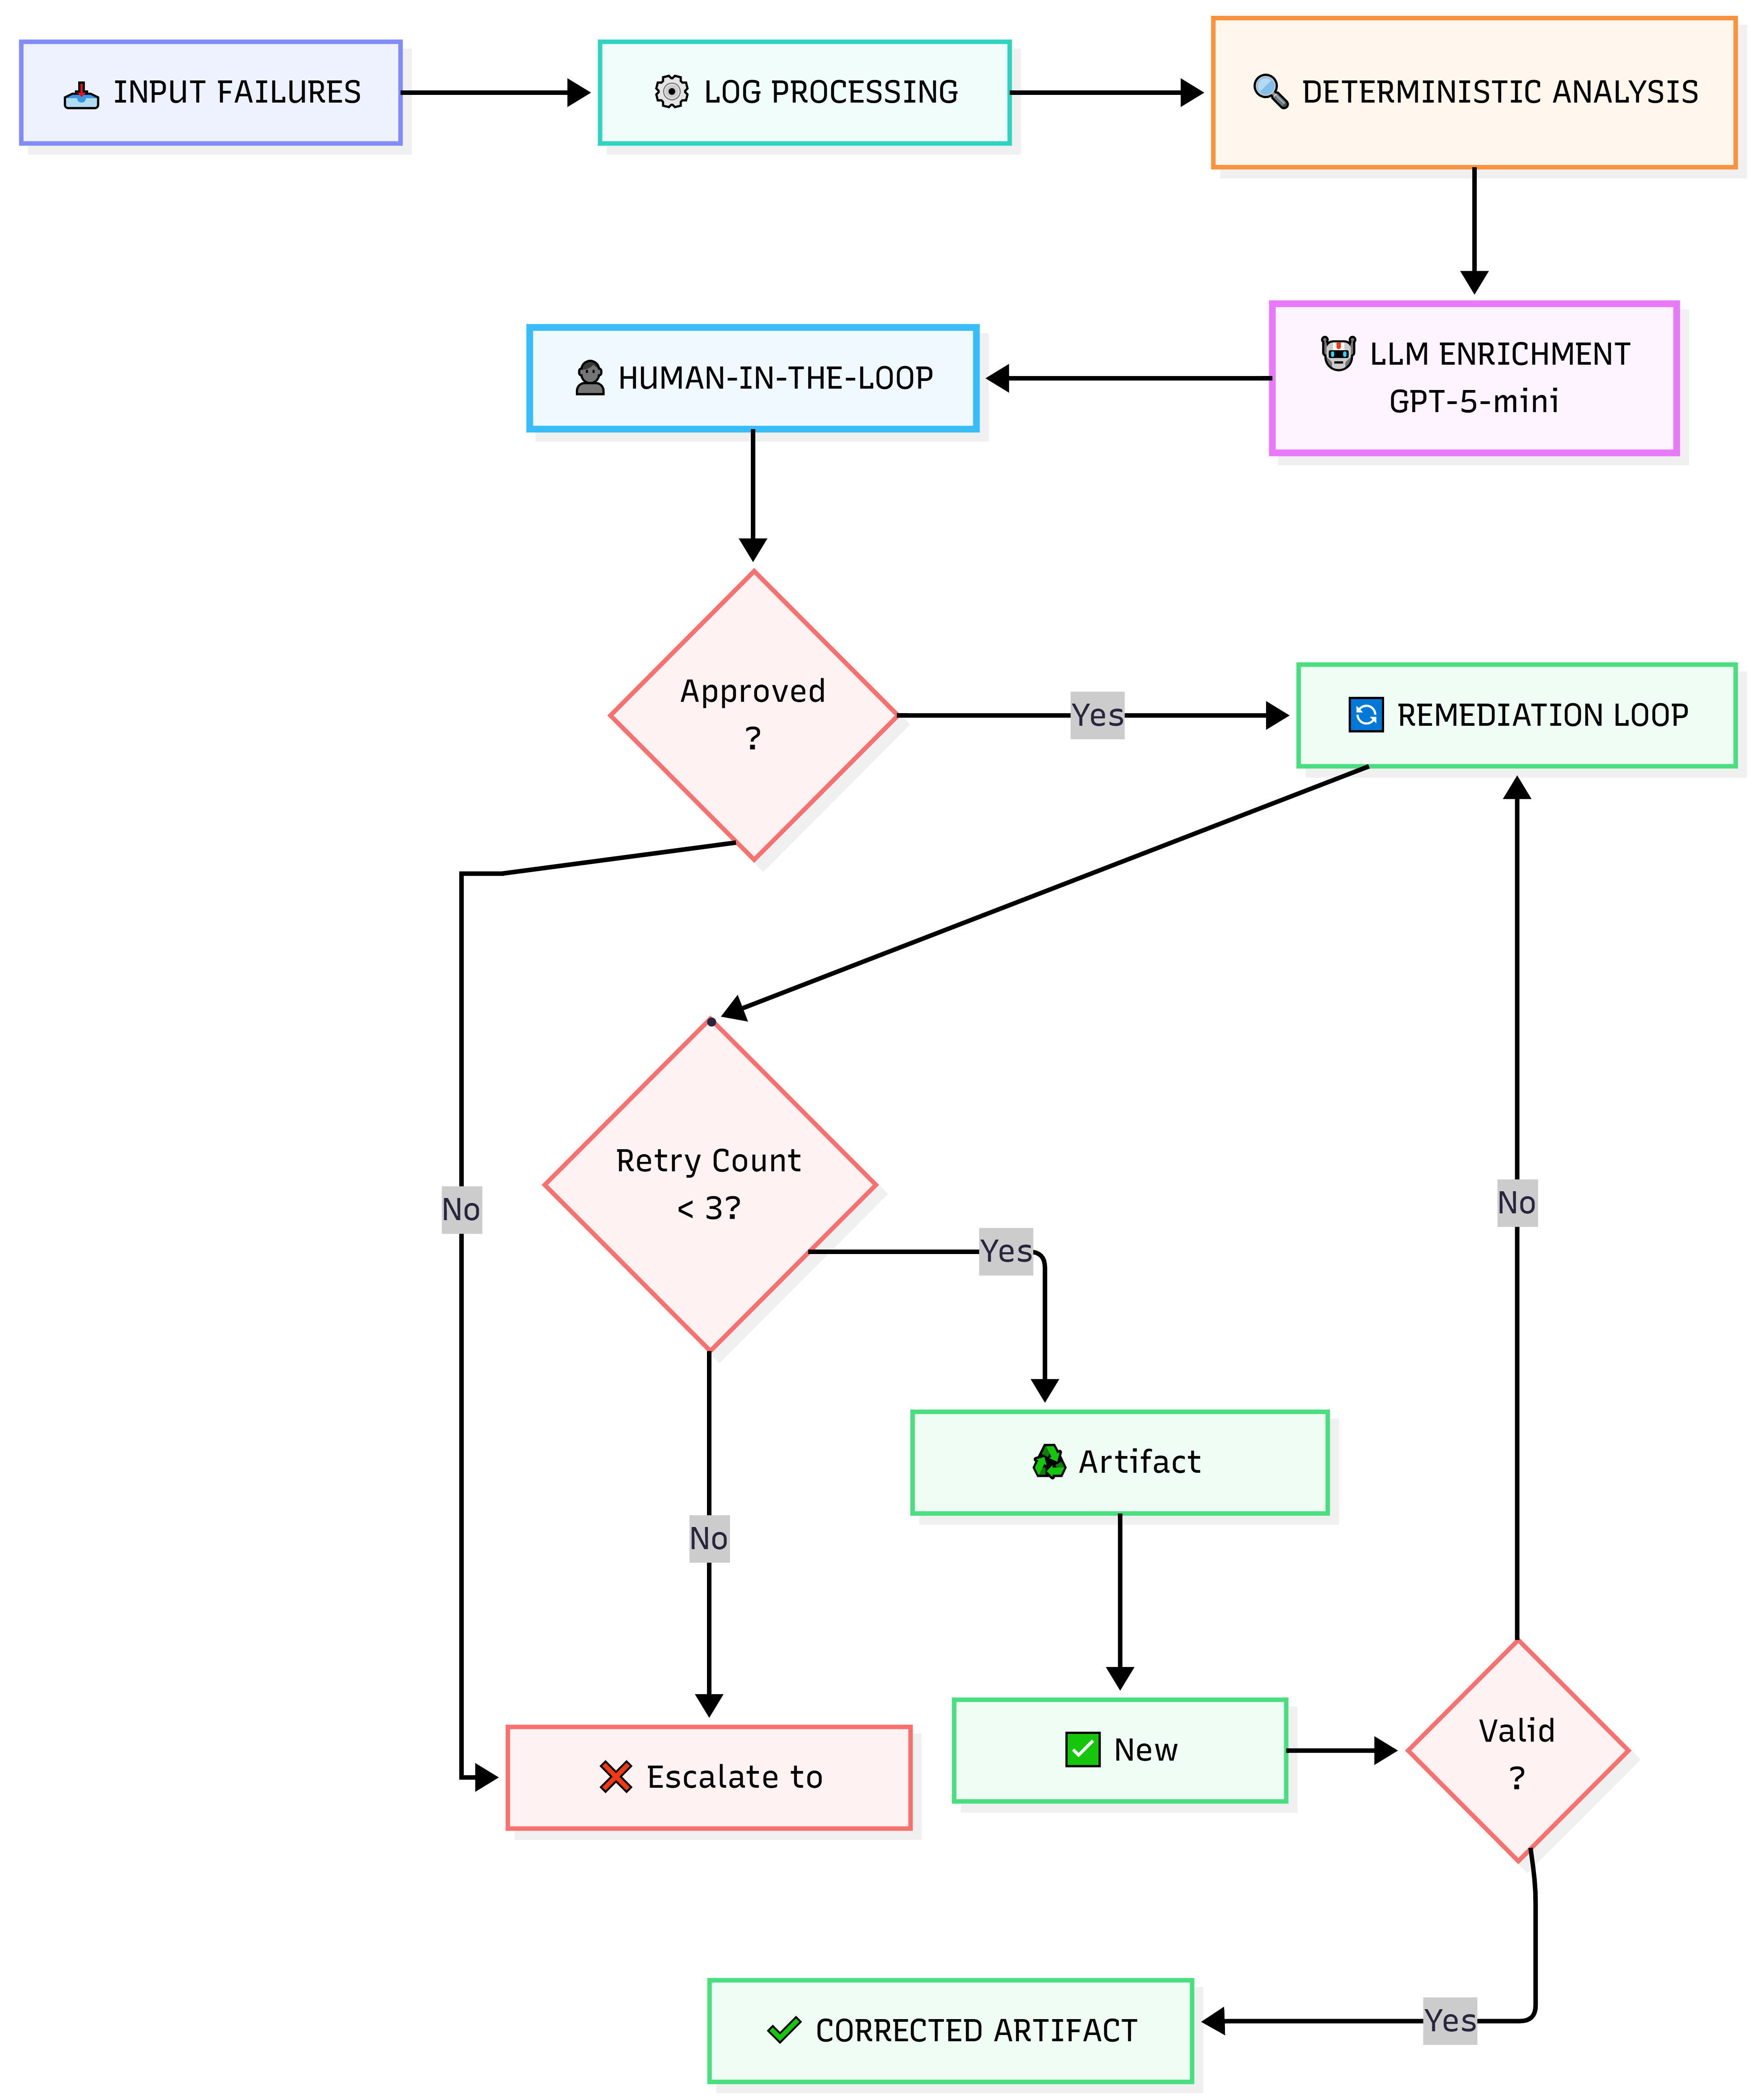
\includegraphics[width=0.85\textwidth]{images/Intelligent Error Remediation.png}
    \caption{Architecture fonctionnelle du \textit{Corrector Agent}}
    \label{fig:corrector-arch}
\end{figure}

Le workflow de la figure~\ref{fig:corrector-arch} repose sur un principe clé~: une analyse
déterministe précède le recours au modèle. Les journaux d'échec sont d'abord normalisés et
classifiés par des règles déterministes~; GPT-5-mini n'intervient qu'ensuite, pour enrichir
le diagnostic et formuler une correction. La proposition est soumise à l'utilisateur
(\textit{human-in-the-loop})~: une fois approuvée, elle alimente une boucle bornée à trois
tentatives qui régénère puis revalide l'artefact. En cas de succès, l'artefact corrigé est
livré~; sinon, ou si la limite est atteinte, le cas est escaladé. Ce séquencement
---~déterminisme d'abord, IA ensuite, validation humaine et boucle bornée~--- limite le
coût des appels au modèle et évite les corrections divergentes.

\begin{itemize}
    \item \textbf{Entrées :} les journaux d'une exécution en échec (build ou validation),
    l'artefact fautif et le contexte du projet associé.
    \item \textbf{Sorties :} un artefact corrigé et validé, ou une escalade documentée
    lorsque la boucle est épuisée, dans les deux cas tracée pour audit.
    \item \textbf{Base de connaissances (RAG) :} une base vectorisée des motifs d'erreurs
    récurrents et de leurs remédiations~; les passages pertinents sont injectés dans le
    contexte du modèle pour ancrer la correction sur des solutions éprouvées.
    \item \textbf{LLM utilisé :} GPT-5-mini, avec repli automatique sur Llama~3.3~70B.
\end{itemize}

\subsubsection{Justification métier}

La remédiation d'erreurs est la tâche la plus exigeante en \textbf{raisonnement} de la
plateforme~: l'agent doit interpréter des journaux hétérogènes, en inférer la cause profonde
et proposer une modification ciblée sans dégrader le reste de l'artefact. C'est cette
capacité d'analyse des logs et de raisonnement causal qui prime ici, et sur laquelle
GPT-5-mini se distingue des modèles légers, au diagnostic souvent superficiel. La régularité
de ses sorties limite en outre le nombre d'itérations de la boucle de correction, où chaque
tentative engage un appel au modèle.

\subsection{Génération d'infrastructure assistée par IA}

L'\textit{Infrastructure Agent} assure le provisionnement automatisé de l'infrastructure
cible~: à partir du contexte projet, il sélectionne une architecture adaptée et génère les
artefacts correspondants, prêts au déploiement.

\subsubsection{Architecture et workflow}

\begin{figure}[htbp]
    \centering
    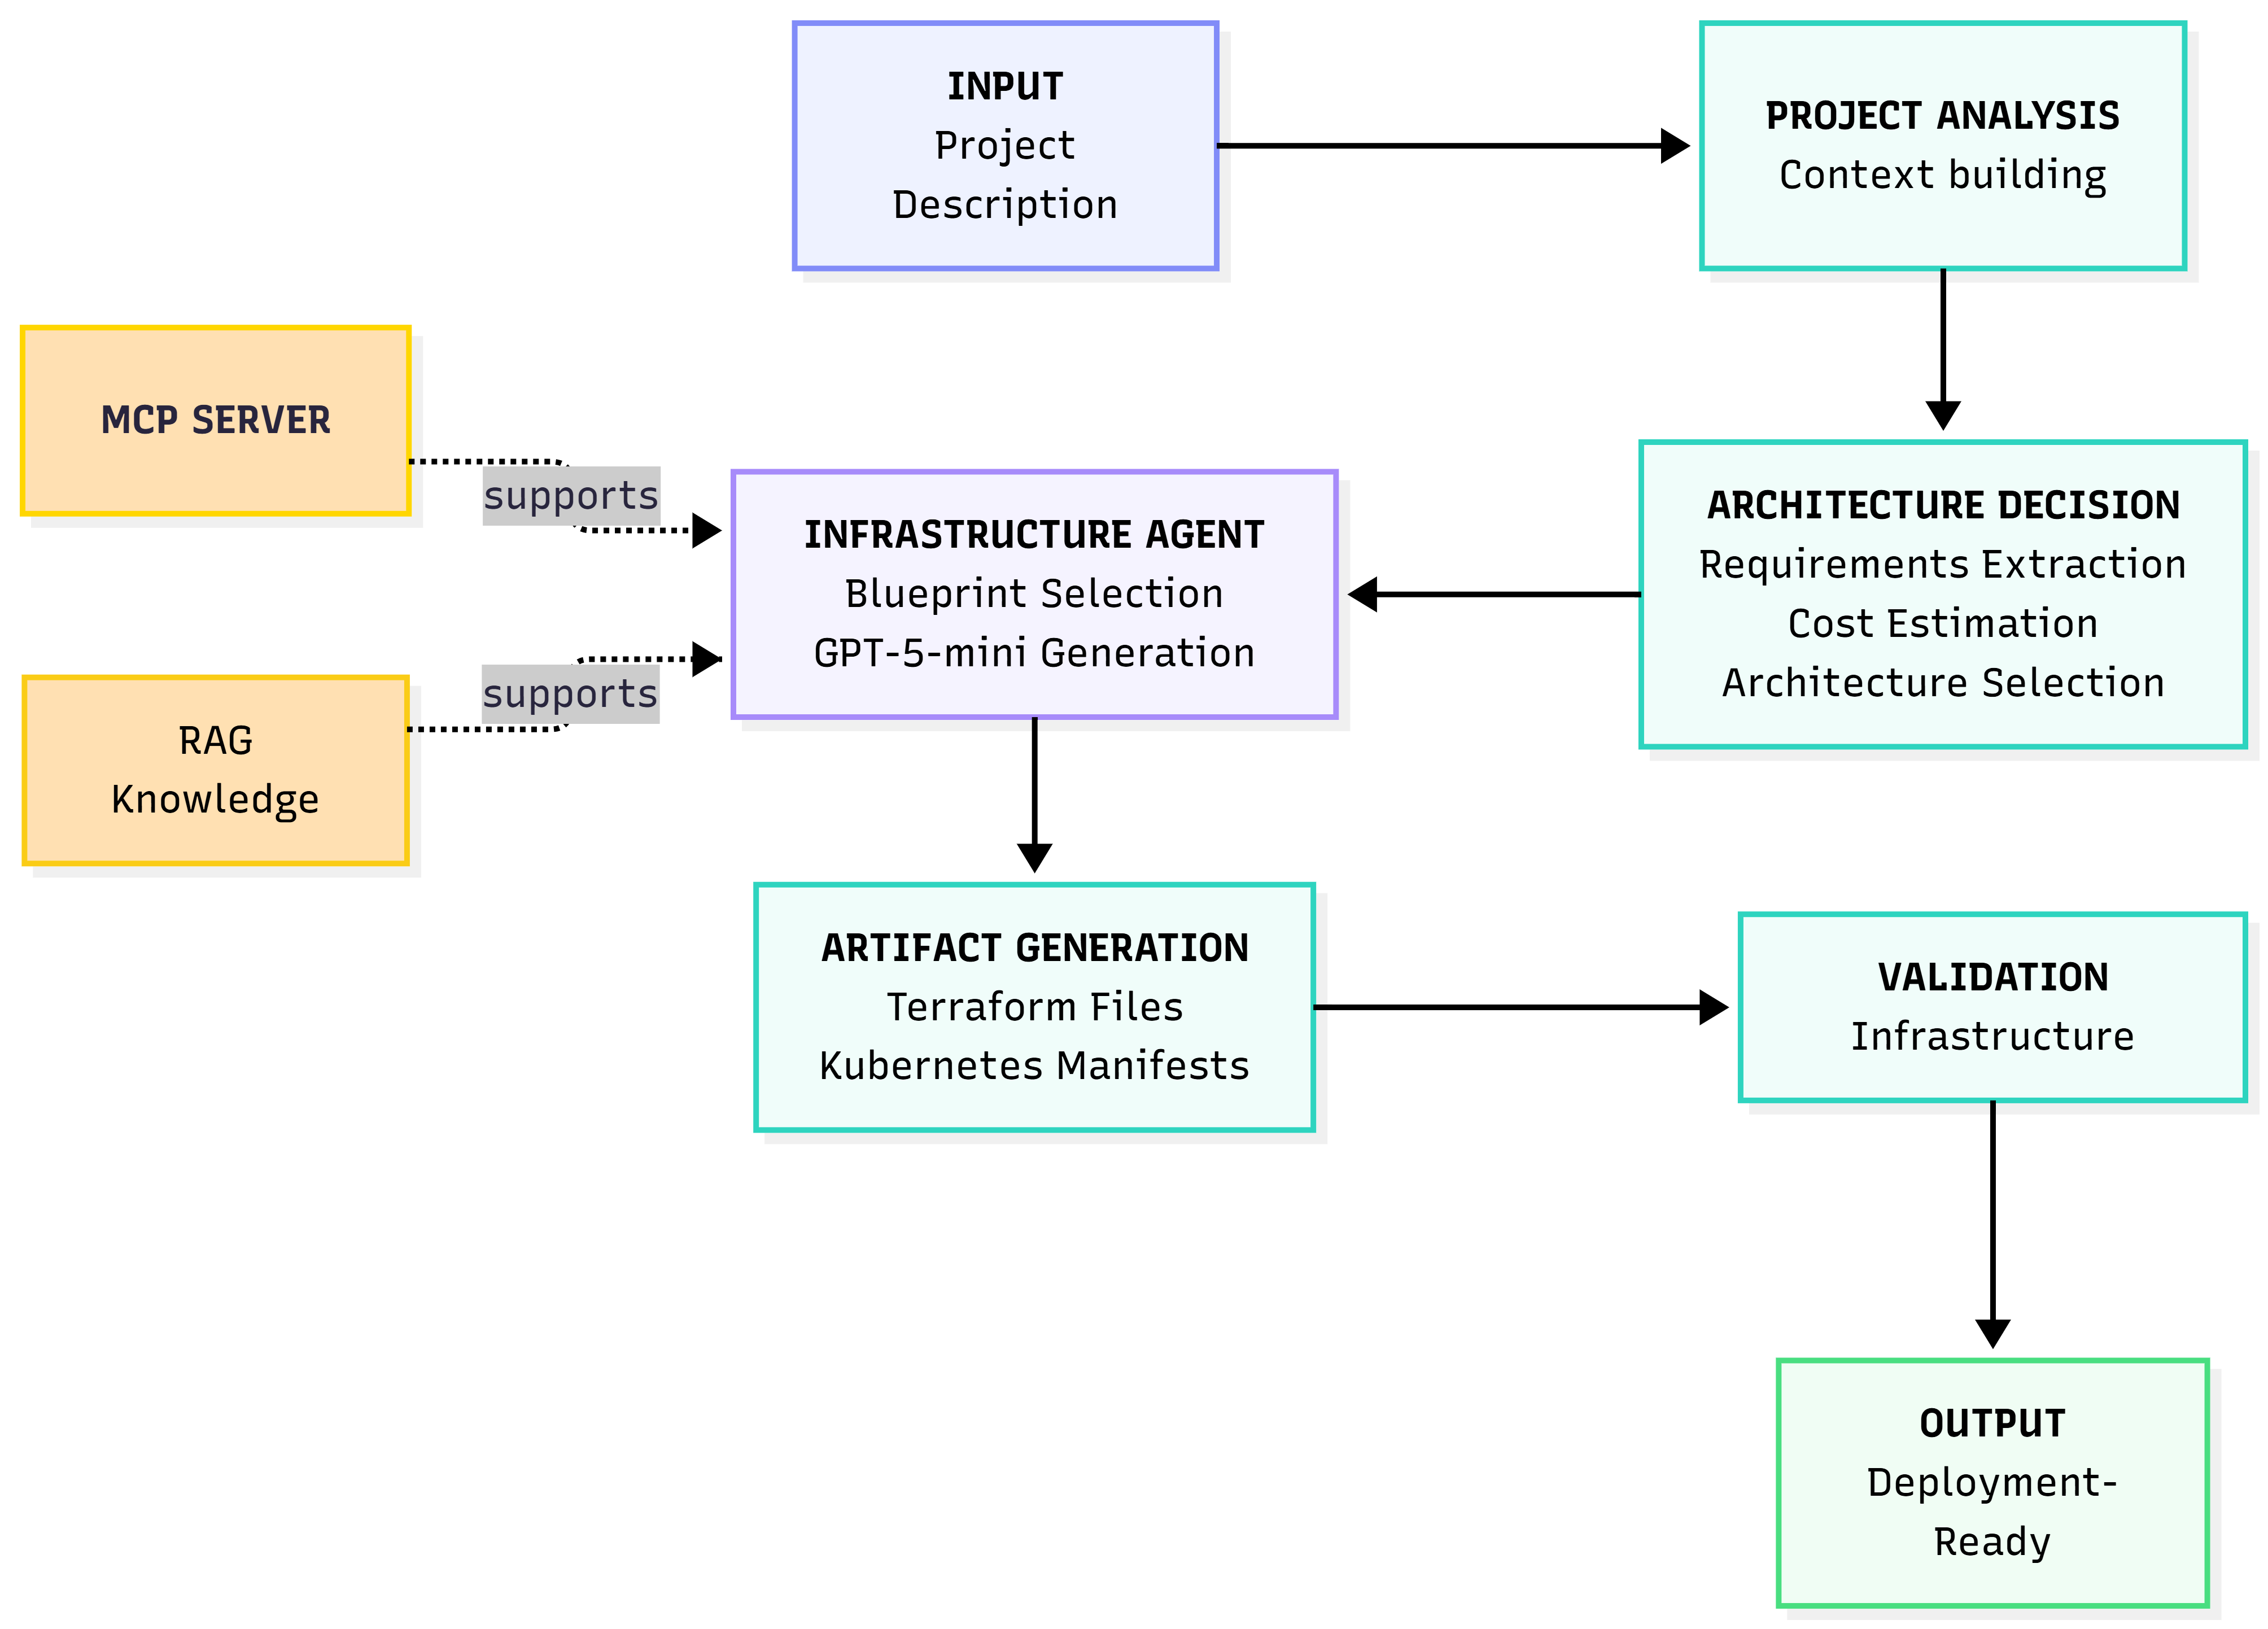
\includegraphics[width=0.90\textwidth]{images/Powered Infrastructure Generation.png}
    \caption{Architecture fonctionnelle de l'\textit{Infrastructure Agent}}
    \label{fig:infra-arch}
\end{figure}

Le workflow de la figure~\ref{fig:infra-arch} sépare trois responsabilités~: la décision,
la génération et la validation. Une phase d'analyse construit d'abord le contexte technique
du projet, puis une étape de décision combine extraction des besoins, estimation des coûts
et sélection de l'architecture la plus pertinente. L'\textit{Infrastructure Agent} exploite
cette décision pour choisir un \textit{blueprint} de référence et piloter la génération.
Deux services encadrent ce raisonnement~: le serveur MCP, qui fournit un accès outillé aux
ressources d'infrastructure, et la base RAG, qui ancre les sorties sur des références
éprouvées. Les artefacts produits sont enfin validés avant de constituer un livrable
déployable, ce qui garantit leur traçabilité et leur fiabilité.

\begin{itemize}
    \item \textbf{Entrées :} la description du projet et son contexte technique (besoins
    applicatifs, contraintes de déploiement, objectifs de coût).
    \item \textbf{Sorties :} des artefacts d'infrastructure validés et prêts au déploiement
    (fichiers Terraform et manifestes Kubernetes).
    \item \textbf{Base de connaissances (RAG) :} une base vectorisée des bonnes pratiques
    Terraform et Kubernetes, complétée par le serveur MCP qui expose les ressources
    d'infrastructure de façon structurée.
    \item \textbf{LLM utilisé :} GPT-5-mini, avec repli automatique sur Llama~3.3~70B.
\end{itemize}

\subsubsection{Justification métier}

La génération d'infrastructure exige des sorties longues, structurées et strictement
conformes à des schémas déclaratifs (HCL, YAML). L'enjeu central est ici le
\textbf{déterminisme}~: une configuration partiellement invalide échoue à la validation et
déclenche des reprises coûteuses. GPT-5-mini a été retenu pour sa capacité à produire des
artefacts valides dès la première passe, ce qui réduit les échecs de validation et fiabilise
l'estimation des coûts associée à l'architecture retenue.

\subsection{Génération de pipelines CI/CD assistée par IA}

Le \textit{CI/CD Agent} automatise la construction des pipelines d'intégration et de
déploiement continus~: à partir du contexte projet et de l'infrastructure définie, il génère
un pipeline complet et validé.

\subsubsection{Architecture et workflow}

\begin{figure}[htbp]
    \centering
    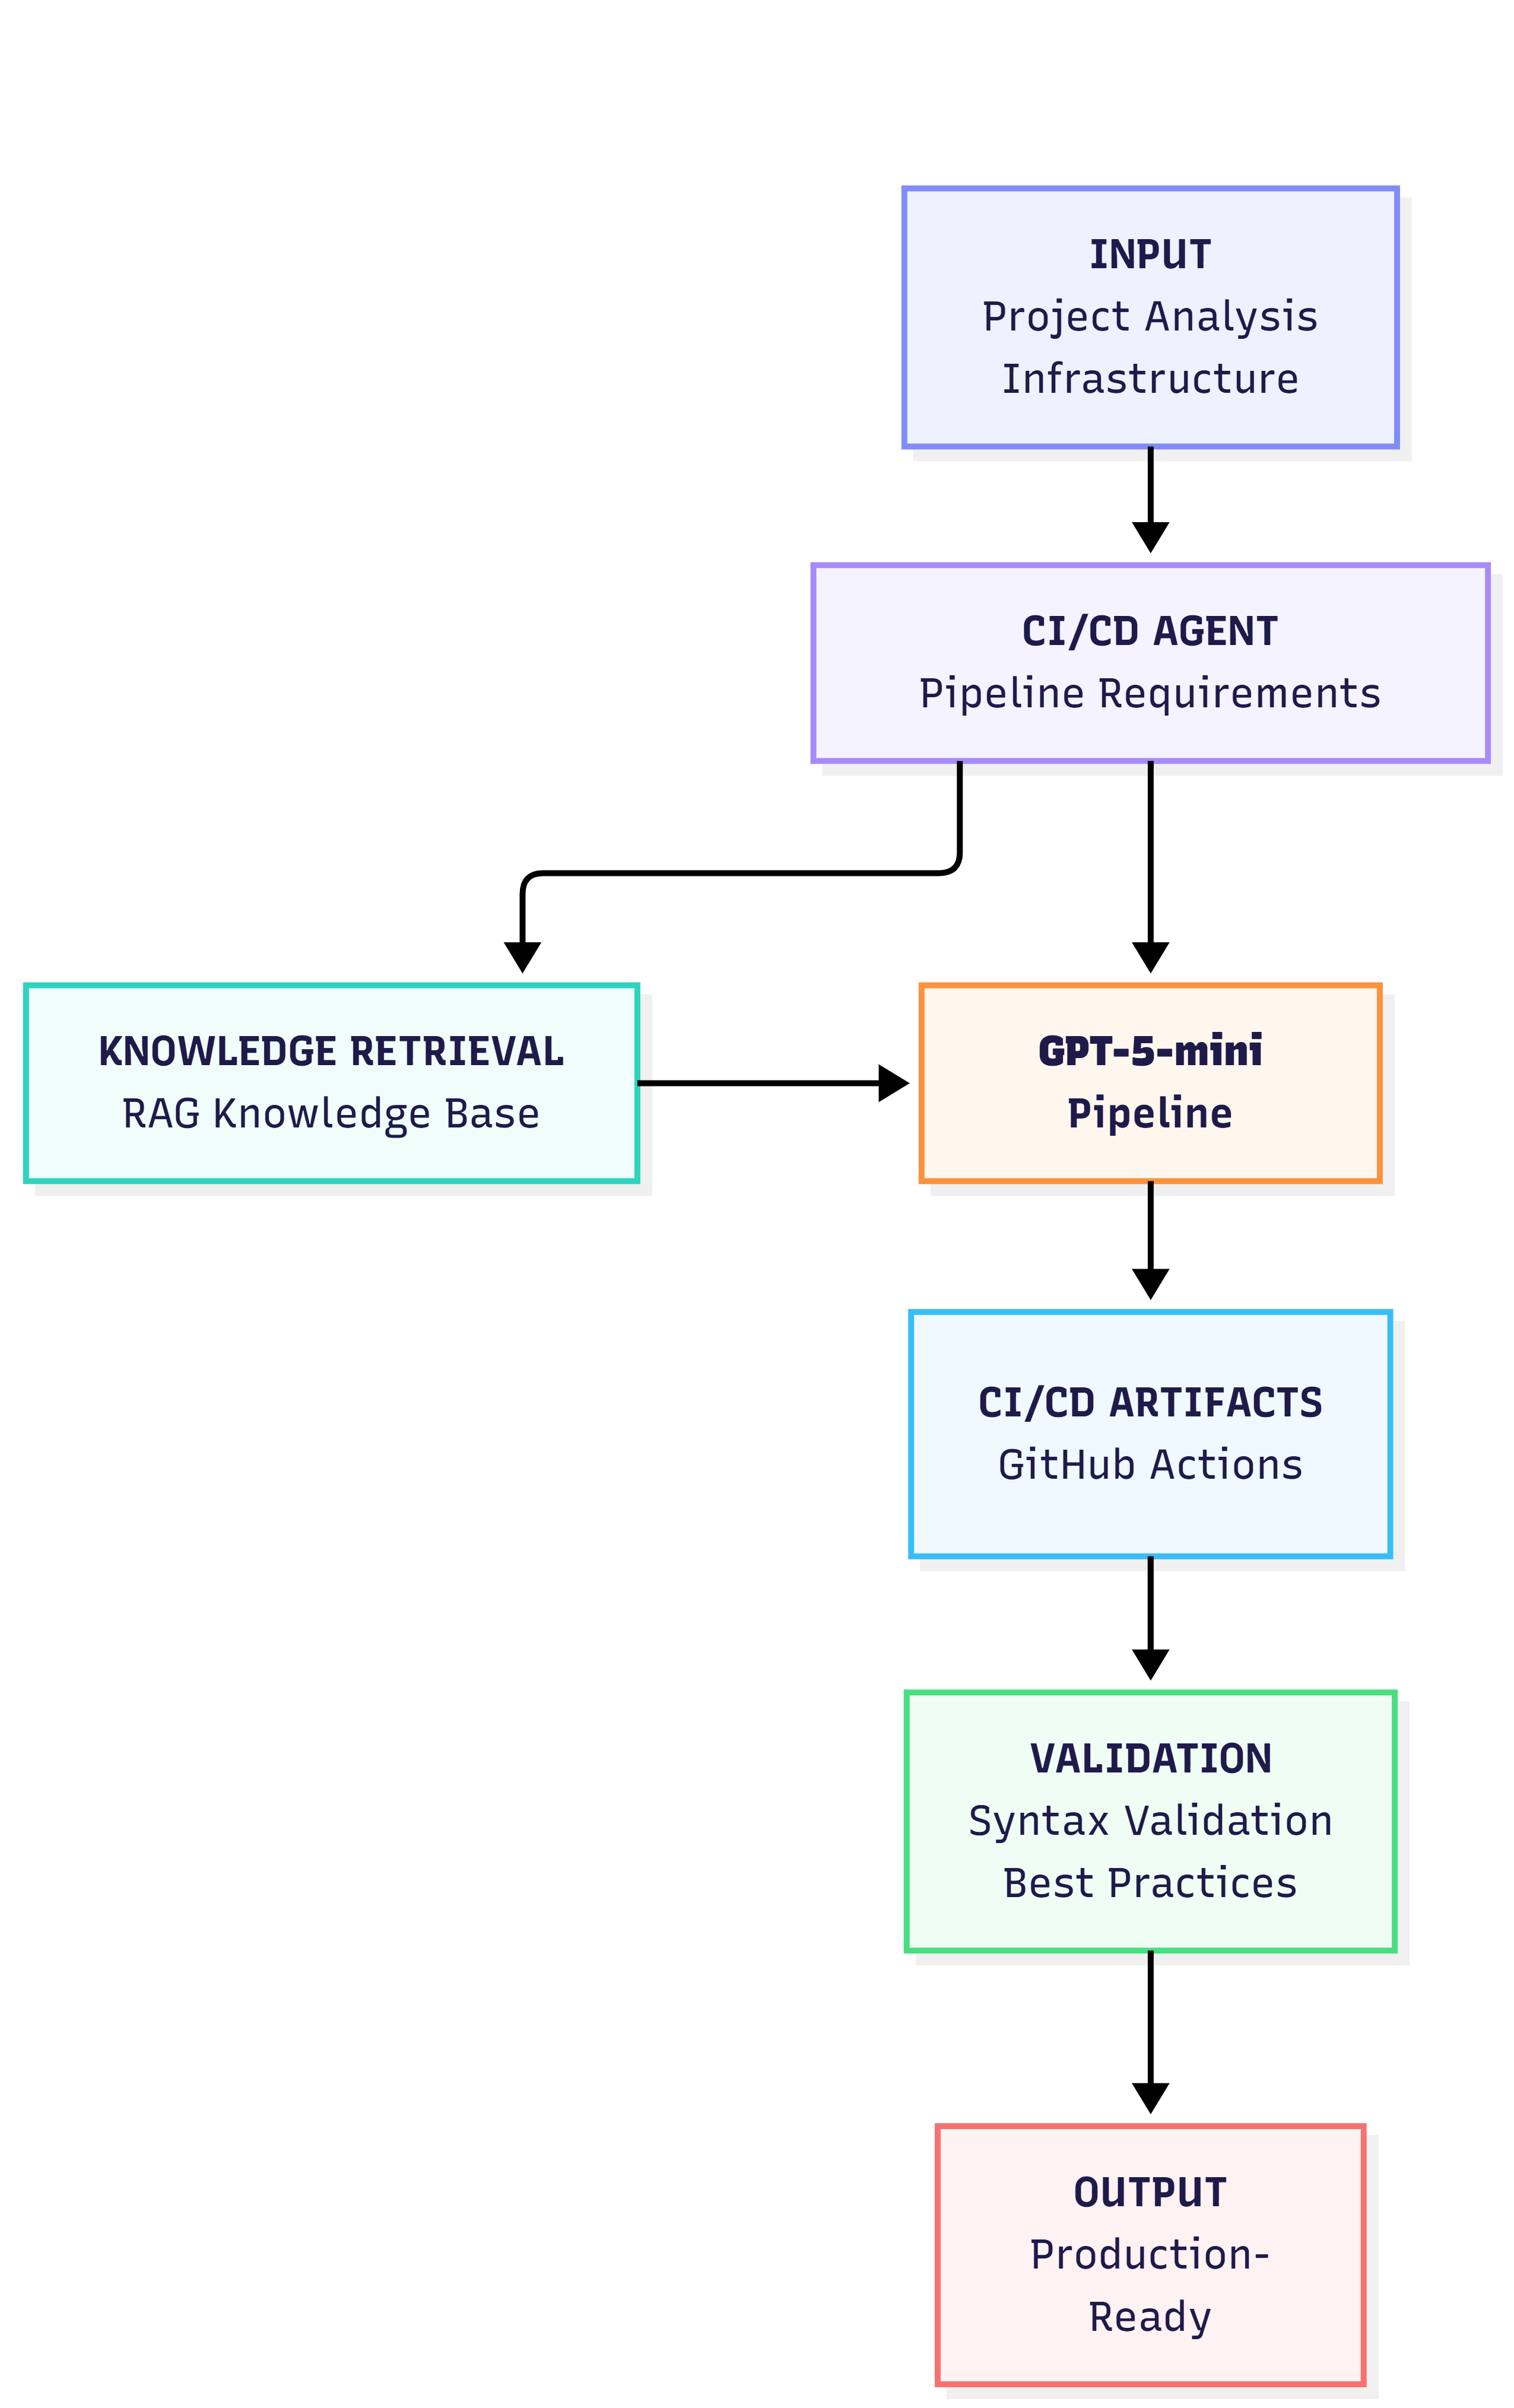
\includegraphics[width=0.72\textwidth]{images/AI-Powered CICD Generation.png}
    \caption{Architecture fonctionnelle du \textit{CI/CD Agent}}
    \label{fig:cicd-arch}
\end{figure}

Le workflow de la figure~\ref{fig:cicd-arch} part du contexte d'analyse du projet et de
l'infrastructure pour dériver les besoins du pipeline. Le \textit{CI/CD Agent} formalise ces
exigences, interroge la base RAG pour récupérer les références pertinentes (étapes de build,
conventions de déploiement) puis pilote la génération. Le pipeline est produit sous forme
d'artefacts CI/CD, avant une étape de validation portant sur la syntaxe et le respect des
bonnes pratiques. Les bonnes pratiques de sécurité sont intégrées directement aux artefacts
générés, comme propriété de qualité du pipeline plutôt que comme contrôle a posteriori.

\begin{itemize}
    \item \textbf{Entrées :} le contexte d'analyse du projet et les caractéristiques de
    l'infrastructure cible précédemment générée.
    \item \textbf{Sorties :} un pipeline CI/CD validé et prêt pour la production (workflows
    GitHub Actions).
    \item \textbf{Base de connaissances (RAG) :} une base vectorisée dédiée aux pratiques
    CI/CD~; les références adaptées sont injectées dans le raisonnement pour aligner les
    pipelines sur les standards de build et de déploiement.
    \item \textbf{LLM utilisé :} GPT-5-mini, avec repli automatique sur Llama~3.3~70B.
\end{itemize}

\subsubsection{Justification métier}

La génération de pipelines CI/CD repose sur la \textbf{cohérence des workflows YAML}~:
l'enchaînement des étapes (build, test, déploiement) doit être correct et les dépendances
entre \textit{jobs} respectées. Au-delà de la validité syntaxique, l'agent doit préserver la
logique globale du pipeline et y intégrer les bonnes pratiques comme propriété de qualité des
artefacts. GPT-5-mini assure cette cohérence de bout en bout avec une régularité supérieure
aux modèles évalués, tout en produisant des définitions YAML valides et maintenables.

\section{Conclusion}

Ce chapitre a formalisé les besoins de la plateforme, puis posé les bases de sa conception à
travers une modélisation UML couvrant les vues fonctionnelle, structurelle et dynamique, et
une architecture globale. Il a enfin détaillé les capacités d'intelligence artificielle qui
en constituent le c\oe ur, en explicitant l'architecture des agents spécialisés et une
méthodologie d'évaluation reposant sur des benchmarks publics, la documentation des
fournisseurs et une approche \textit{LLM-as-a-Judge}. Ces choix obéissent à une logique
commune~--- ancrage documentaire par RAG et fournisseur de raisonnement mutualisé
(GPT-5-mini, avec repli sur Llama~3.3~70B)~--- déclinée selon les exigences métier de chaque
agent. Le chapitre suivant présente la réalisation effective de la plateforme.
